\subsection*{h. Una lista con la venta promedio, venta total, mayor venta, menor venta, y total de órdenes, por región, estado y ciudad. La venta promedio debe estar entre \$ 900 y \$1,500.}

Para este ejercicio, primero obtendremos una tabla con los elementos necesarios para realizar los cálculos. Para esto, por cada región, estado y ciudad, necesitamos conocer cada orden realizada y el valor de la venta.

Posteriormente, podemos usar la tabla del paso anterior y agrupar sus tuplas en base a la región, estado y ciudad, agregando además nuevas columnas para los valores que podemos calcular a partir de las órdenes y los valores realizados. 
\begin{itemize}
    \item Para el promedio usamos avg() sobre las ventas y la columna 'promedio'
    \item Para el máximo usamos max() sobre las ventas y la columna 'ventamaxima'
    \item Para el mínimo usamos min() sobre las ventas y la columna 'ventaminima' 
    \item Para la cantidad de órdenes, usamos count() sobre orderid y la columna 'totalordenes'
\end{itemize}

Finalmente, usamos la tabla anterior para escoger solo aquellos elementos en los que el promedio está entre \$ 900 y \$1500

Así, obtenemos la expresión:
\begin{equation}
\begin{split}
&\sigma_{\text{promedio} \geq 900 \land \text{promedio} \leq 1500} \Biggl( \gamma_{\substack{\text{region, state, city}; \\ \text{AVG(venta)} \to \text{promedio}, \text{SUM(venta)} \to \text{ventas}, \\ \text{MAX(venta)} \to \text{ventamaxima}, \text{MIN(venta)} \to \text{ventaminima}, \\ \text{COUNT(orderid)} \to \text{totalordenes}}} \\
&\Biggl( \left( \pi_{\substack{\text{customerid, orderid,} \\ \text{venta} \leftarrow \text{quantity} * \text{price}}} ( \text{orders} \bowtie \text{products} ) \right) \bowtie \text{customer} \Biggr) \Biggr) 
\end{split}
\end{equation}

Resultados obtenidos:

\begin{figure}[H]
    \centering
    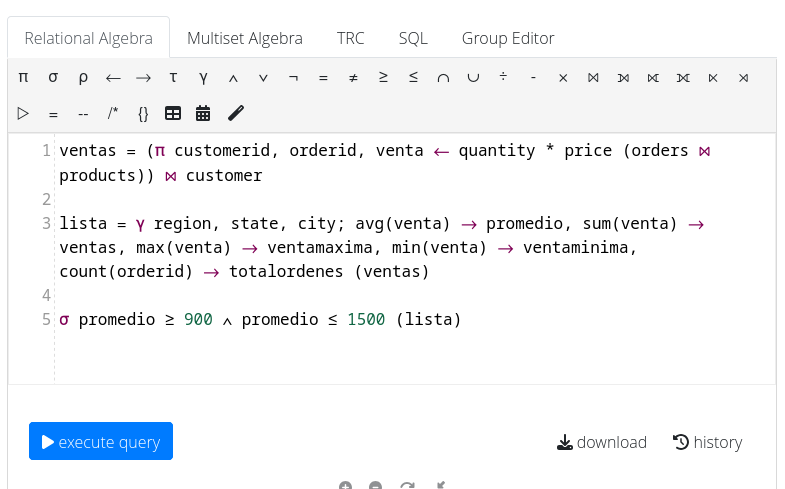
\includegraphics[width=0.7\textwidth]{imagenes/2.h-Query.png}
    \caption{Consulta}
\end{figure}

\begin{figure}[H]
    \centering
  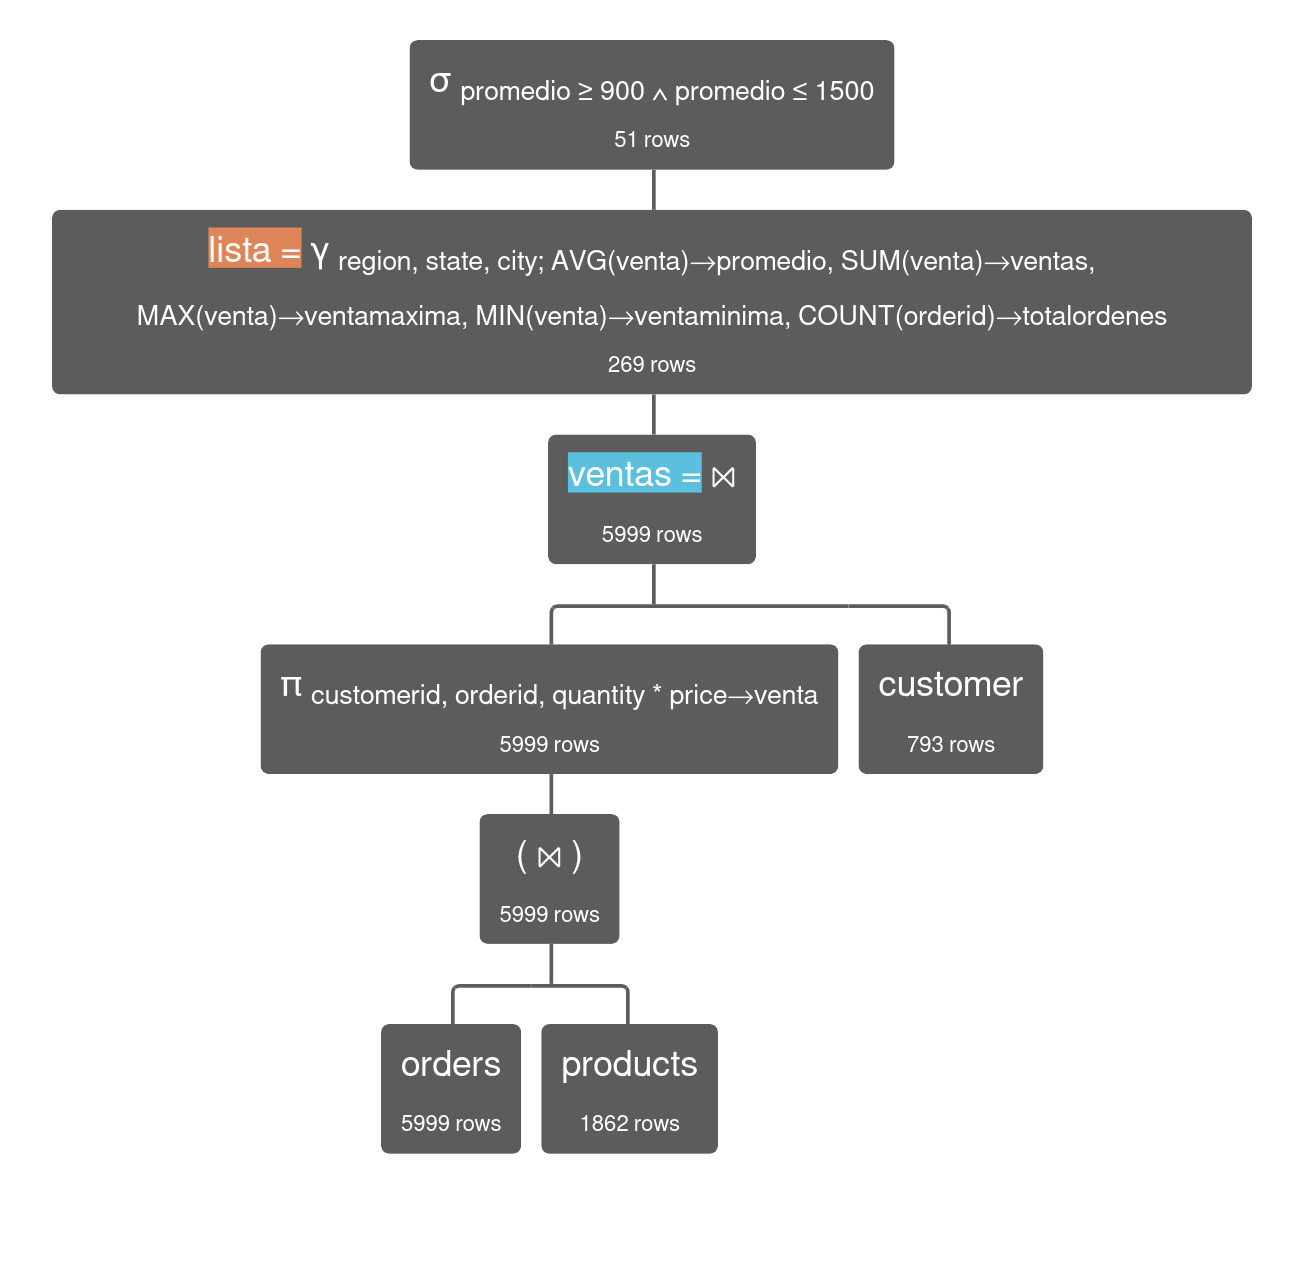
\includegraphics[width=0.7\textwidth]{imagenes/2.h-Three.png}
    \caption{Árbol de consulta.}
\end{figure}

    
\begin{figure}[H]
    \centering
  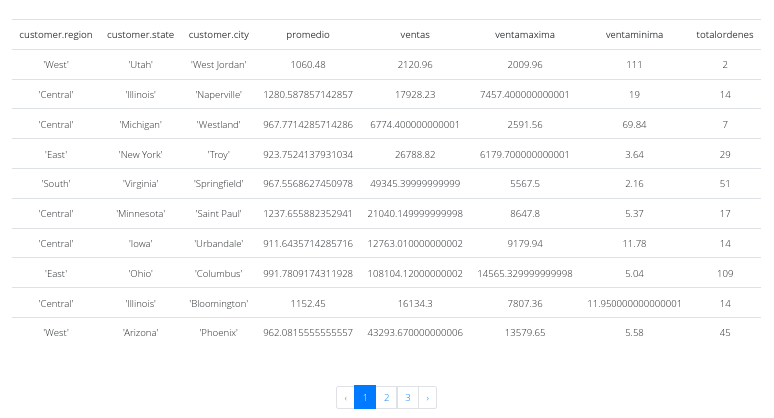
\includegraphics[width=0.7\textwidth]{imagenes/2.h-Tabla.png}
    \caption{Resultado de consulta.}
\end{figure}
